%==================================================
%      PREAMBOLO e DICHIARAZIONI INIZIALI
%==================================================
\documentclass[10pt,oneside,a4paper]{article}

\usepackage[latin1]{inputenc} 
\usepackage[italian]{babel}
\usepackage[T1]{fontenc}
\usepackage{siunitx} %Inserisce automaticamente i dati con le unit�  di misura correttamente formattate del SI (utilizzo: \SI{0.82}{m^2}, in generale \SI{misura con il punto decimale}{unit�  di misura})
\sisetup{output-decimal-marker = {.}, separate-uncertainty = true, input-uncertainty-signs = \pm, detect-weight=true, detect-family=true} %per usare SI con il punto decimale
\usepackage{listings} %Per citare codice informatico formattandolo correttamente
\usepackage{amsmath,amsthm,verbatim,amssymb,amsfonts,amscd, graphicx,mathtools}
\usepackage[makeroom]{cancel}
\newcommand{\abs}[1]{\left\lvert\,#1\,\right\rvert}
\usepackage{geometry}
\usepackage{epigraph}
\usepackage{booktabs}	%tabelle migliorate
\usepackage{tablefootnote}	%note a pi� di pagina in tabella
\usepackage{threeparttable} %tabella con note a pi� di tabella
\usepackage{caption}	%descrizione per figure
\usepackage{dblfnote}
\captionsetup{tableposition=top,figureposition=bottom,font=small} %setup descrizione
\usepackage{float}
\usepackage{esvect} %vettori
\usepackage{longtable} %tabelle lunghe
\usepackage[dvipsnames]{xcolor}
\definecolor{sepia}{HTML}{80002A}
\usepackage[colorlinks=true, citecolor=black, linkcolor=sepia, urlcolor=black]{hyperref}
\usepackage{mathrsfs}
\usepackage{circuitikz}


\usepackage{multicol}
\newenvironment{Figure}
  {\par\medskip\noindent\minipage{\linewidth}}
  {\endminipage\par\medskip}

\newcommand{\var}{\operatorname{var}}
\newcommand{\cov}{\operatorname{cov}}


\usepackage{listings} %Per inserire codice
\lstnewenvironment{codice_c}[1][]
{\lstset{basicstyle=\small\ttfamily, columns=fullflexible,
keywordstyle=\color{red}\bfseries, commentstyle=\color{blue},
language=C, basicstyle=\small,
numbers=left, numberstyle=\tiny,
stepnumber=2, numbersep=5pt, frame=shadowbox,  showstringspaces=false, #1}}{}

%==================================================
%                  PRIMA PAGINA
%==================================================

\title{\textsc{\textbf{Esercitazione 2}: Amplificatore ad emettitore comune}}
\author{\small{G. Galbato Muscio} \and \small{L. Gravina} \and \small{L. Graziotto}}
\date{\today}

\begin{document}
	\begin{figure}
		\centering
		
\includegraphics[scale=0.5, trim={2.8cm 8.9cm 0 9cm}, clip]{logo.png}
	\end{figure}
	\maketitle
	\begin{center} 
		\fbox{{\fontsize{12pt}{8mm}\textsc{Gruppo 11}}} \\
	\end{center}
\hrule
\vspace{0.5cm}
\renewcommand{\abstractname}{Abstract}
\begin{abstract}
Si utilizza un transistor 2N2222A di tipo \emph{npn} per realizzare un amplificatore ad emettitore comune, con amplificazione di tensione di circa $A_v = -50$. Se ne studia quindi la risposta in frequenza e le resistenze in uscita e in ingresso.
\end{abstract}
\vspace{4cm}
\tableofcontents %Indice
\newpage


\pagebreak
\begin{multicols}{2}
%==================================================
%      		PROGETTO RETE AUTOPOLARIZZANTE
%==================================================
\section{Progetto della rete autopolarizzante}
Si realizza il circuito seguente per l'amplificatore, utilizzando un transistor 2N2222A di tipo \emph{npn}.

\begin{flushleft}
\hspace*{-1cm}
\begin{circuitikz} [scale=.9]
	\draw (0,0) node[ground]{}
	(0,0) to[sV, l=$v_{\text{s}}$] (0,2) to[R=$R_s$] (1.5,2) to[C=$C_1$] (3.5,2)
	(1.75,2) node[circ]{} node[above]{$v_i$}
	(3.5,-0.5) to[R=$R_2$] (3.5,2)
	(3.5,2) to[R=$R_1$] (3.5,4.5)
	(5,2) node[npn] (npn) {}
	(3.5,2) -- (npn.B);
	\draw (5,-0.5) to[R=$R_E$] (npn.E);
	\draw (npn.C) to[R=$R_C$] (5,4.5);
	\draw (npn.C) to[C=$C_2$] ++(1.5,0) to[short, -*] ++(0.25,0) node[right] {$v_o$};
	\draw (npn.E) -- ++(1,0) to[C=$C_E$] (6,-0.5)
	(6,-0.5) -- (5,-0.5)
	(3.5,4.5) -- (5,4.5)
	(3.5,-0.5) -- (5,-0.5)
	(4.25,4.5) to[short, *-] (4.25,4.75) node[above] {$V_\text{CC}$}
	(4.25,-0.5) node[ground]{}
	;\end{circuitikz}
\end{flushleft}

Si vuole ottenere un'amplificazione di $A_v \simeq -50$, dunque si scelgono resistenze di valore prossimo a quello indicato nel progetto della guida all'esperienza. Poich� i valori disponibili saranno diversi, tuttavia, si proceder� a verificare la correttezza dell'amplificazione ottenuta, calcolando direttamente i valori previsti e confrontandoli con quelli misurati sul circuito.
I valori degli elementi utilizzati sono, come da misura con il multimetro e con il ponte:
\begin{equation*}
\begin{aligned}
R_1 &= \SI{32.8 \pm 0.2}{k\ohm} \\
R_2 &= \SI{8.22 \pm 0.04}{k\ohm} \\
R_C &= \SI{1.174 \pm 0.006}{k\ohm} \\
R_E &= \SI{1.188 \pm 0.006}{k\ohm} \\
V_\text{CC} &= \SI{9.967 \pm 0.005}{V} \\
C_1 &= \SI{42.31 \pm 0.02}{nF} \\
C_2 &= \SI{155.34 \pm 0.08}{nF} \\
C_E &= \SI{89.62 \pm 0.05}{\micro F}.
\end{aligned}
\end{equation*}
Si verifica con il multimetro che le tensioni tra i diversi nodi del circuito siano compatibili con quelle previste, dati gli elementi usati, al fine di verificare il corretto funzionamento del circuito stesso. 

Si ha, nell'ipotesi che il circuito si trovi nella regione attiva\footnote{Dunque si ha $V_\text{BE} = 0.7$ e $I_B$ trascurabile; si verificher� la correttezza di queste ipotesi}:
\begin{equation*}
\begin{aligned}
V_\text{BB} &= \frac{R_2}{R_1+R_2}V_\text{CC} \\
V_\text{B} &\simeq V_\text{BB} \\
I_C &= \frac{V_\text{BB} - V_\text{BE}}{R_E} \\
I_E &\simeq I_C \\
V_C &= V_\text{CC} - R_C I_C \\
V_\text{CE} &= V_\text{CC} - (R_E + R_C)I_C \\
V_\text{E} &= V_C - V_\text{CE}
\end{aligned}
\end{equation*}

Per quanto riguarda le correnti di emettitore e di collettore, che nella regione attiva devono essere circa uguali, si misura con il multimetro la differenza di potenziale ai capi di $R_C$ e $R_E$ e si applica la legge di Ohm $I = V/R$. Si riporta in tabella~\ref{tab:verifica} il confronto tra valore previsto e misurato.

\begin{center}
\captionof{table}{Valori previsti e misurati per il circuito}
\label{tab:verifica}
\begin{tabular}{l|c|c}
 & Valore previsto & Valore misurato \\
\hline
$V_C$ & \SI{8.68}{V} & \SI{8.67 \pm 0.04}{V}\\
$V_B$ & \SI{1.998}{V} & \SI{1.95 \pm 0.01}{V}\\
$V_E$ & \SI{1.3}{V} & \SI{1.315 \pm 0.007}{V}\\
$V_\text{CE}$ & \SI{7.39}{V} & \SI{7.36 \pm 0.04}{V}\\
$V_\text{BE}$ & \SI{0.7}{V} & \SI{0.632 \pm 0.003}{V}\\
$I_C$ & \SI{1.09}{mA} & \SI{1.10 \pm 0.01}{mA}\\
$I_E$ & \SI{1.09}{mA} & \SI{1.11 \pm 0.01}{mA}\\
\hline
\end{tabular}
\end{center}

Dalla tabella si evince che la differenza di potenziale tra base ed emettitore � compatibile con il valore $V_\text{BE} = \SI{0.7}{V}$, e la differenza di potenziale tra collettore ed emettitore � $V_\text{CE} > \SI{0.2}{V}$, dunque il transistor si trova nella regione attiva. L'amplificazione prevista risulta essere 
\begin{equation}\label{eq:amp}
A_v = -\frac{R_C I_C}{V_T} = -51.7 \pm 0.5,
\end{equation}
dove $V_T = \SI{25}{mV}$ alla temperatura del laboratorio, ed � compatibile con il valore richiesto dal progetto.

Al fine di stabilizzare il punto di lavoro, si introducono i condensatori $C_1$, $C_2$ e $C_E$: i primi due impediscono le variazioni delle correnti statiche dovute alla connessione del generatore di segnali e della resistenza di carico, mentre $C_E$ permette di ottenere un'amplificazione data da~(\ref{eq:amp}) invece che da $A_v = -R_C / R_E$, per frequenze sufficientemente alte. La scelta compiuta per la $C_E$ verifica la condizione
\[
\frac{1}{\omega C_E} \ll R_E
\]  
anche per pulsazioni molto basse, dell'ordine di $10/(R_E C_E) \sim \SI{93.9}{s^{-1}}$, ossia fino a circa \SI{15}{Hz}.
Utilizzando i condensatori $C_1$ e $C_2$, scelti con capacit� molto grandi al fine di aumentare il pi� possibile la banda passante dell'amplificatore, si introdurranno comunque delle frequenze di taglio
\begin{equation}\label{eq:freqTaglio}
\begin{aligned}
f' &= \frac{1}{2\pi C_1 R_\text{in}} \\
f'' &= \frac{1}{2\pi C_2 (R_\text{out} + R_L)},
\end{aligned}
\end{equation}
dove $R_\text{in} = R_B || h_\text{ie} \simeq R_B$\footnote{Dal datasheet del transistor si ha $h_\text{ie} = 2 \div 8$ \SI{}{k\ohm}.} e $R_\text{out} = R_C || h_\text{oe}^{-1} \simeq R_C$\footnote{Sempre dal datasheet del transistor, si ha infatti $h_\text{oe} = 5\div35$ \SI{}{\micro \ohm^{-1}}.}, mentre $R_L$ sar� la resistenza di carico introdotta nel seguito.


%==================================================
%      		DINAMICA DEL CIRCUITO
%==================================================
\section{Dinamica del circuito}
Si connette al circuito il generatore di segnali e si imposta un segnale sinusoidale con frequenza fissa di \SI{53.6 \pm 1.6}{kHz} e ampiezza variabile $v_s$; si ricorda che la resistenza interna del generatore $R_s \simeq \SI{50}{\ohm}$ viene trascurata. Si connette inoltre al canale \texttt{CH1} dell'oscilloscopio il segnale d'ingresso e al canale \texttt{CH2} il segnale $v_o$.
Variando $v_s$, si misura con l'oscilloscopio l'ampiezza picco-picco di $v_i$ e di $v_o$, e si stima l'amplificazione $A_v = -v_o / v_i$. Si riportano in tabella~\ref{tab:dinamica} i valori misurati.

\begin{center}
\captionof{table}{Misure di ampiezza picco-picco di $v_i$ e $v_o$}
\label{tab:dinamica}
\begin{tabular}{c|c|c}
$v_i$ [\SI{}{mV}] ($\pm 3\%$) & $v_o$ ($\pm 3\%$) [\SI{}{V}] & $A_v$ \\
\hline
		19.80 &        0.91 &   46.06 \\
        26.40 &        1.21 &   45.83 \\
        34.00 &        1.55 &   45.59 \\
        39.20 &        1.90 &   48.47 \\
        47.60 &        2.20 &   46.22 \\
        56.00 &        2.56 &   45.71 \\
        62.00 &        2.82 &   45.48 \\
        72.00 &        3.24 &   45.00 \\
        84.00 &        3.68 &   43.81 \\
\hline
\end{tabular}
\end{center}

Si ha un'amplificazione media di
\[
A_v = 45.8 \pm 1.2.
\]
Si osserva che per ampiezze superiori a $v_i \simeq \SI{90}{mV}$, il segnale appare distorto: questo � dovuto alla limitata dinamica del transistor. Si riporta in figura~\ref{fig:distorsione} uno screenshot dell'oscilloscopio per evidenziare il fenomeno.

\begin{figure}[H]
	\begin{center}
	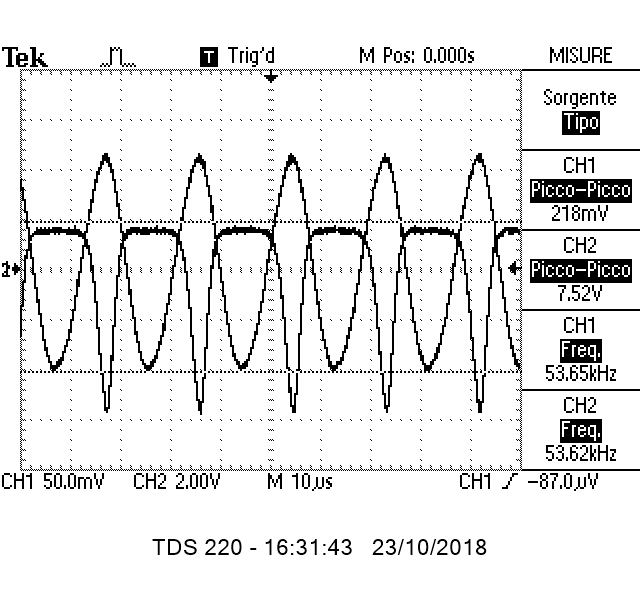
\includegraphics[width=\linewidth]{taglio2.png}
	\caption{Distorsione del segnale per elevati valori di $v_i$}
	\label{fig:distorsione}
	\end{center}
\end{figure}


%==================================================
%      		STUDIO IN FREQUENZA
%==================================================
\section{Studio in frequenza}
Si procede allo studio in frequenza del circuito, variando anche $v_s$ per evitare nella misura i fenomeni di distorsione precedentemente descritti. Si riporta in tabella~\ref{tab:frequenza} i valori di frequenza, $v_i$, $v_o$ e del modulo dell'amplificazione $\abs{A_v} = \abs{v_o} / \abs{v_i}$, e in figura~\ref{fig:bode} il diagramma di Bode corrispondente. 

\begin{figure}[H]
	\begin{center}
	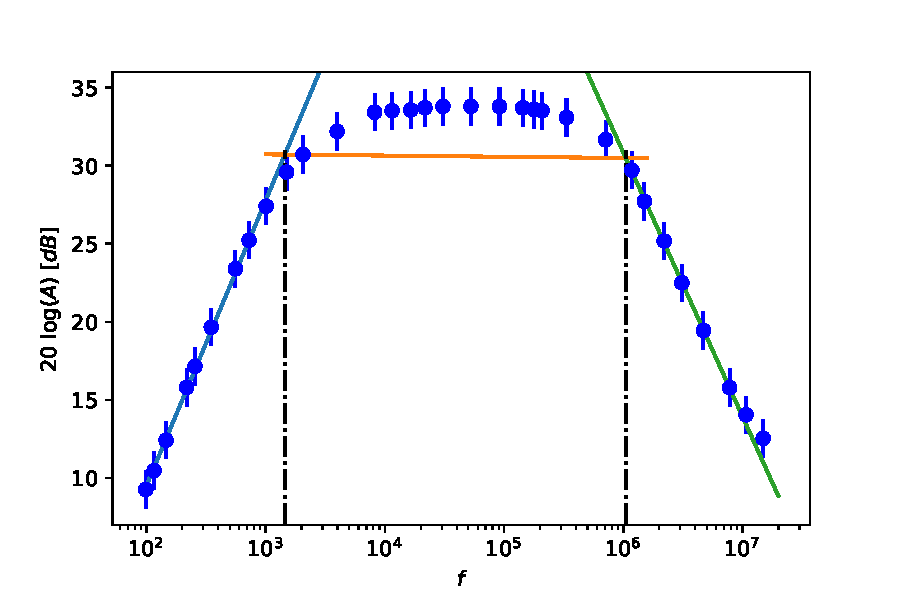
\includegraphics[width=\linewidth]{bode_rette.pdf}
	\caption{Diagramma di Bode dell'amplificazione in funzione della frequenza}
	\label{fig:bode}
	\end{center}
\end{figure}

Si osserva che per frequenze superiori ai \SI{10}{MHz} l'andamento dell'amplificazione in funzione della frequenza segue una pendenza diversa da quella precedentemente assunta dall'inizio della zona decrescente. Si ritiene che questo sia dovuto all'intervento della capacit� interna dell'oscilloscopio, che si aggiunge ai gi� presenti effetti capacitativi parassiti del transistor.

Si stimano quindi le frequenze di taglio inferiori e superiori, mediante un fit nelle tre zone dei punti che presentano un andamento lineare crescente, stazionario e decrescente, e trovando le intersezioni di quella crescente e decrescente con la retta stazionaria traslata verso il basso di \SI{3}{\dB}, ovvero del valore assunto in decibel dall'amplificazione alla frequenza di taglio. Si ha 
\[
\begin{aligned}
f_L &= \SI{1.45 \pm 0.07}{kHz} \\
f_H &= \SI{1.05 \pm 0.05}{MHz};
\end{aligned}
\]
si confronta la prima con le frequenze di taglio delle~(\ref{eq:freqTaglio}), ovvero $f' = \SI{1199 \pm 21}{Hz}$, $f'' = \SI{1.02 \pm 0.02}{Hz}$ e con $f_E = 1/(2\pi C_E R_E) = \SI{1.49 \pm 0.01}{Hz}$ e si evince che nella zona crescente si ha l'effetto del solo filtro passa-alto dovuto a $C_1$, dal momento che le frequenze di taglio degli altri due filtri sono di molto inferiori; questo � visibile anche dalla pendenza della retta, pari a \SI{20}{\dB} per decade. Per la frequenza di taglio superiore, invece, poich� essa � dovuta alle capacit� parassite del transistor ignote, non si � in grado di fornire un valore teorico di confronto. 

\end{multicols}
\begin{table*}
\captionof{table}{Studio in frequenza dell'amplificatore}
\label{tab:frequenza}
\begin{center}
\begin{tabular}{c|c|c|c}
$f$ [\SI{}{Hz}] & $v_i$ ($\pm 3\%$) [\SI{}{mV}] & $v_o$ [\SI{}{mV}] ($\pm 3\%$) & $\abs{A_v}$ \\
\hline
   9.88e+01 &         39.2 &          114 &  2.91 \\
   1.16e+02 &         39.2 &          131 &  3.34 \\
   1.46e+02 &         39.2 &          164 &  4.18 \\
   2.18e+02 &         36.6 &          226 &  6.17 \\
   2.55e+02 &         39.4 &          284 &  7.21 \\
   3.50e+02 &         36.8 &          354 &  9.62 \\
   5.58e+02 &         39.2 &          580 & 14.80 \\
   7.26e+02 &         36.8 &          672 & 18.26 \\
   1.01e+03 &         39.2 &          920 & 23.47 \\
   1.50e+03 &         36.8 &         1110 & 30.16 \\
   2.06e+03 &         39.0 &         1340 & 34.36 \\
   3.98e+03 &         38.8 &         1580 & 40.72 \\
   8.20e+03 &         38.8 &         1820 & 46.91 \\
   1.15e+04 &         38.8 &         1840 & 47.42 \\
   1.65e+04 &         38.8 &         1850 & 47.68 \\
   2.17e+04 &         38.8 &         1880 & 48.45 \\
   3.07e+04 &         38.8 &         1900 & 48.97 \\
   5.27e+04 &         38.8 &         1900 & 48.97 \\
   9.15e+04 &         38.8 &         1900 & 48.97 \\
   1.43e+05 &         38.8 &         1880 & 48.45 \\
   1.77e+05 &         38.8 &         1860 & 47.94 \\
   2.08e+05 &         38.8 &         1840 & 47.42 \\
   3.34e+05 &         38.8 &         1750 & 45.10 \\
   7.10e+05 &         37.6 &         1440 & 38.30 \\
   1.18e+06 &         36.6 &         1120 & 30.60 \\
   1.50e+06 &         36.2 &          880 & 24.31 \\
   2.20e+06 &         35.8 &          650 & 18.16 \\
   3.10e+06 &         32.4 &          432 & 13.33 \\
   4.70e+06 &         32.6 &          306 &  9.39 \\
   7.80e+06 &         27.6 &          170 &  6.16 \\
   1.07e+07 &         22.6 &          114 &  5.04 \\
   1.49e+07 &         31.6 &          134 &  4.24 \\
\hline
\end{tabular}
\end{center}
\end{table*}
\begin{multicols}{2}

%==================================================
%      		RESISTENZA IN USCITA
%==================================================
\section{Resistenza di uscita}
Si misura la resistenza di uscita dell'amplificatore, inserendo una resistenza di carico $R_L$ tra il potenziale $v_o$ e la terra. Si lavora in regime sinusoidale a frequenza \SI{10.7 \pm 0.3}{kHz} e si fissa innanzitutto il potenziale $v_o = \SI{1.70 \pm 0.05}{V}$ a vuoto, scegliendo $v_i = \SI{36.0 \pm 1.1}{mV}$. Si sceglieranno valori di $R_L \simeq R_C$ per ottimizzare la qualit� della misura, e si varier� tale resistenza misurando la tensione ai suoi capi. Si riportano in tabella~\ref{tab:resistUscita} i valori di $R_L$ e di $v_{R_L}$. Si stima $R_\text{out}$ con
\[
R_\text{out} = \frac{v_o - v_{R_L}}{v_{R_L}}R_L.
\]

\begin{center}
\captionof{table}{Valori misurati per la resistenza di uscita}
\label{tab:resistUscita}
\begin{tabular}{c|c|c}
$R_L$ ($\pm 0.5\%$) [\SI{}{k\ohm}] & $v_{R_L}$ ($\pm 3\%$) [\SI{}{mV}] & $R_\text{out}$ [\SI{}{k\ohm}] \\
\hline
          0.817 &          672.00 &          1.250 \\
          1.770 &         1000.00 &          1.239 \\
          1.510 &          936.00 &          1.233 \\
          1.186 &          840.00 &          1.214 \\
          1.000 &          768.00 &          1.214 \\
\hline
\end{tabular}
\end{center}

La stima della resistenza, data dal valore medio, � dunque
\[
R_\text{out} = \SI{1229 \pm 14}{\ohm},
\]
compatibile con il valore della resistenza $R_C$.

%==================================================
%      		RESISTENZA IN INGRESSO
%==================================================
\section{Resistenza di ingresso}
Si valuta anche la resistenza in ingresso dell'amplificatore, mediante l'inserimento di una resistenza $r_x$ dell'ordine del \SI{}{k\ohm} tra il generatore di segnali e il condensatore $C_1$. Misurando i potenziali $v_i$ e $v_2$ rispettivamente prima e dopo la resistenza $r_x$ con l'oscilloscopio, si ricava il valore della resistenza di ingresso dall'equazione del partitore di tensione:
\[
R_\text{in} = \frac{v_2}{v_i - v_2}r_x.
\]
Si lavora ancora in regime sinusoidale a frequenza \SI{10.7 \pm 0.3}{kHz}.

Si riporta in tabella~\ref{tab:resistIngresso} i valori di $r_x$ e dei potenziali, nonch� le stime di $R_\text{in}$.

La stima della resistenza, data dal valore medio, �
\[
R_\text{in} = \SI{3.25 \pm 0.12}{k\ohm};
\]
si confronta questo valore con quello ricavato dalla frequenza di taglio stimata, ossia $R_\text{in} = 1 /(2\pi f_L C_1) = \SI{2.59 \pm 0.08}{k\ohm}$, e si osserva che sono compatibili, tenendo conto che anche la stima stessa della frequenza di taglio � affetta da incertezza.

\end{multicols}
\begin{table}[H]
\captionof{table}{Valori misurati per la resistenza di ingresso}
\label{tab:resistIngresso}
\centering
\begin{tabular}{c|c|c|c}
$r_x$ ($\pm 3\%$) [\SI{}{k\ohm}] & $v_{i}$ ($\pm 3\%$) [\SI{}{mV}] &  $v_{2}$ ($\pm 3\%$) [\SI{}{mV}]  & $R_\text{in}$ [\SI{}{k\ohm}] \\
\hline
       	  1.000 &            260 &            200 &             3.333 \\
          0.816 &            258 &            208 &             3.396 \\
          1.190 &            262 &            190 &             3.140 \\
          1.510 &            262 &            176 &             3.090 \\
          1.770 &            258 &            168 &             3.304 \\
\hline
\end{tabular}
\end{table}
\begin{multicols}{2}

\end{multicols}
\end{document}